Lo primero fue armar el banco óptico. En un extremo colocamos la fuente de luz y, justo enfrente, la máscara con la rendija, de forma que de toda la luz de la lámpara solo saliera una franja delgada, como se ve en la figura \ref{fig:fuente}.

\begin{center}
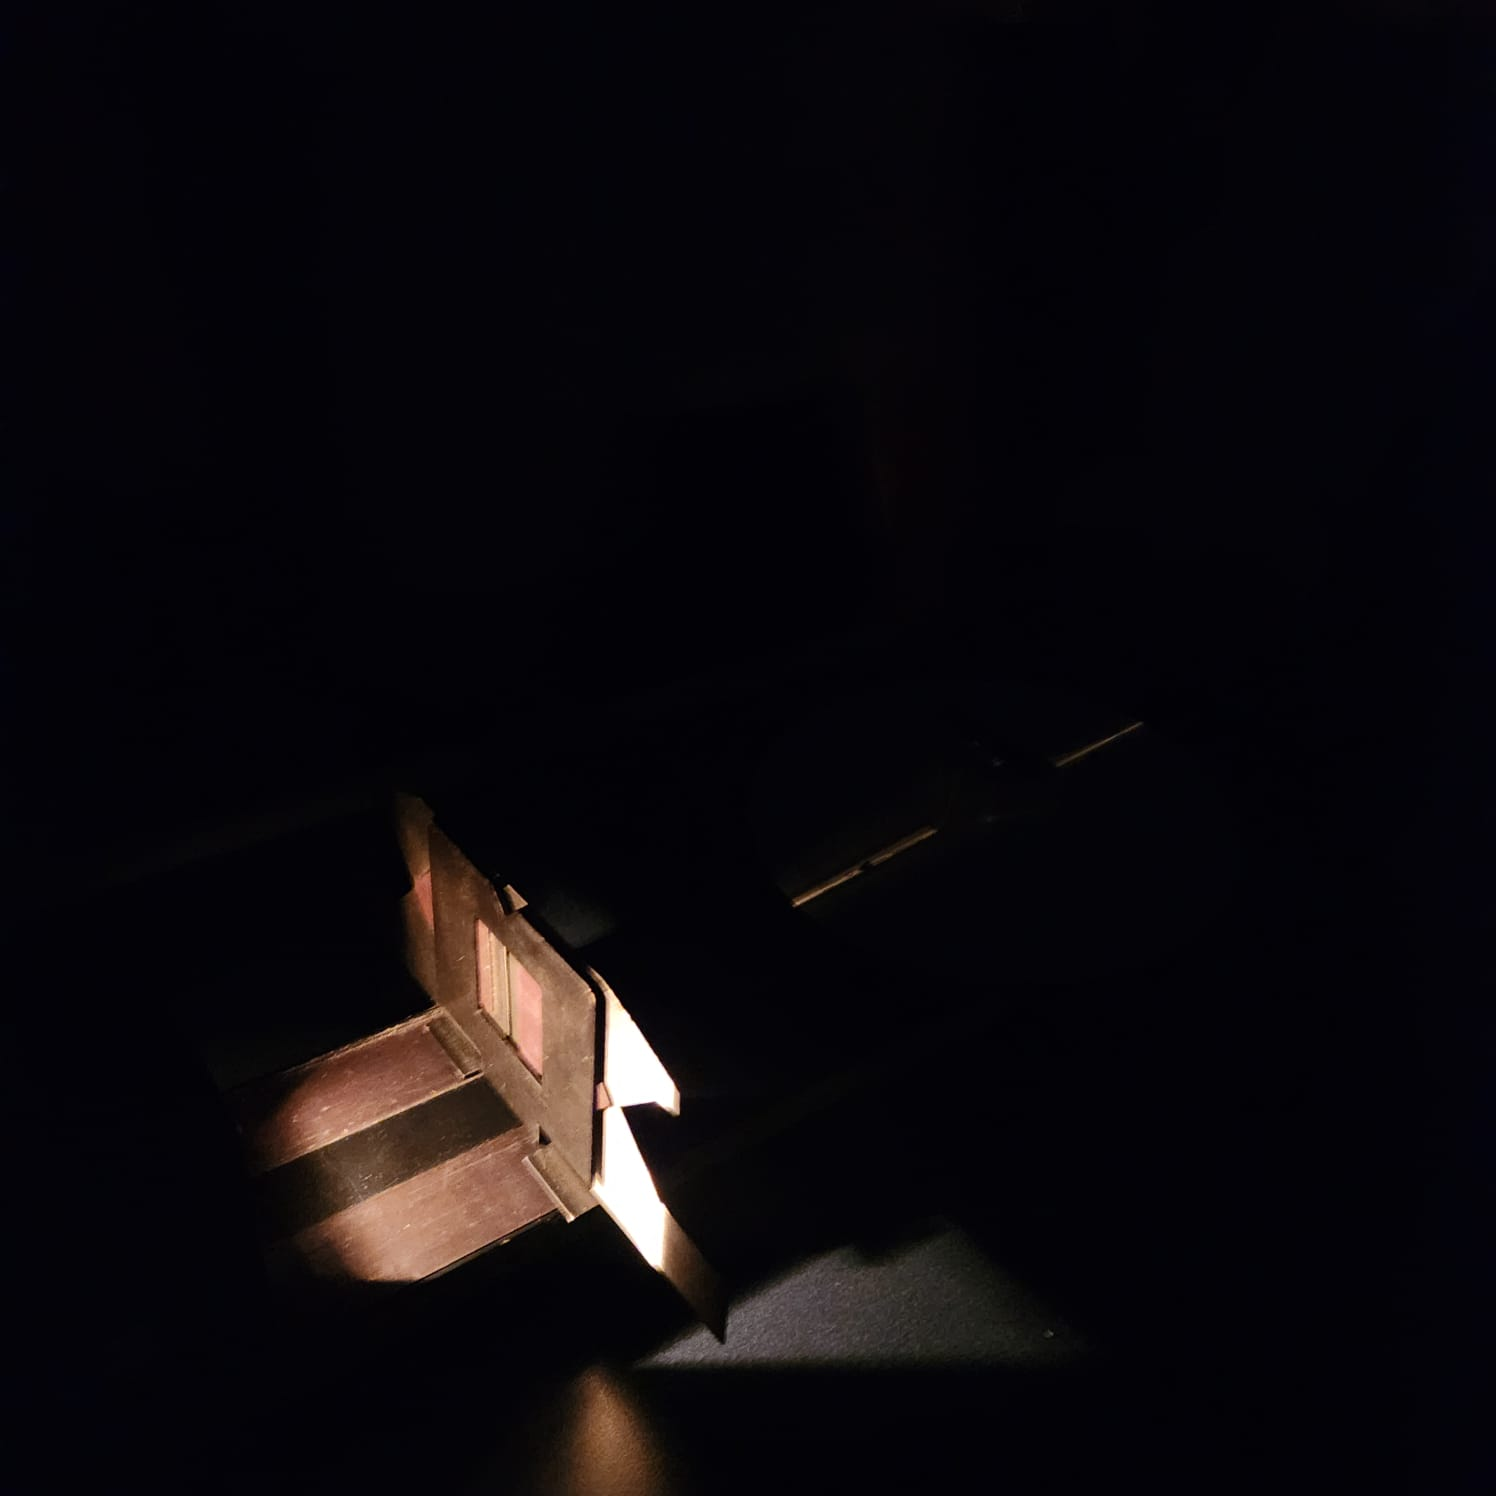
\includegraphics[width=\columnwidth]{fuente_luz.jpg}
\captionof{figure}{Fuente de luz con la máscara de rendija sobre el banco óptico, en el laboratorio a oscuras.}
\label{fig:fuente}
\end{center}

Del otro lado pusimos la mesa de rayos.

Sobre ella acomodamos la lente de acrílico con su cara plana sobre la línea marcada como COMPONENT y con el centro de esa cara en el centro de la mesa. Luego apagamos las luces y alineamos todo hasta que el rayo pasara por la línea NORMAL de la escala y cruzara la lente sin desviarse, porque así sabíamos que el cero estaba bien puesto. La figura \ref{fig:mesa} muestra la mesa ya montada en el banco.

\begin{center}
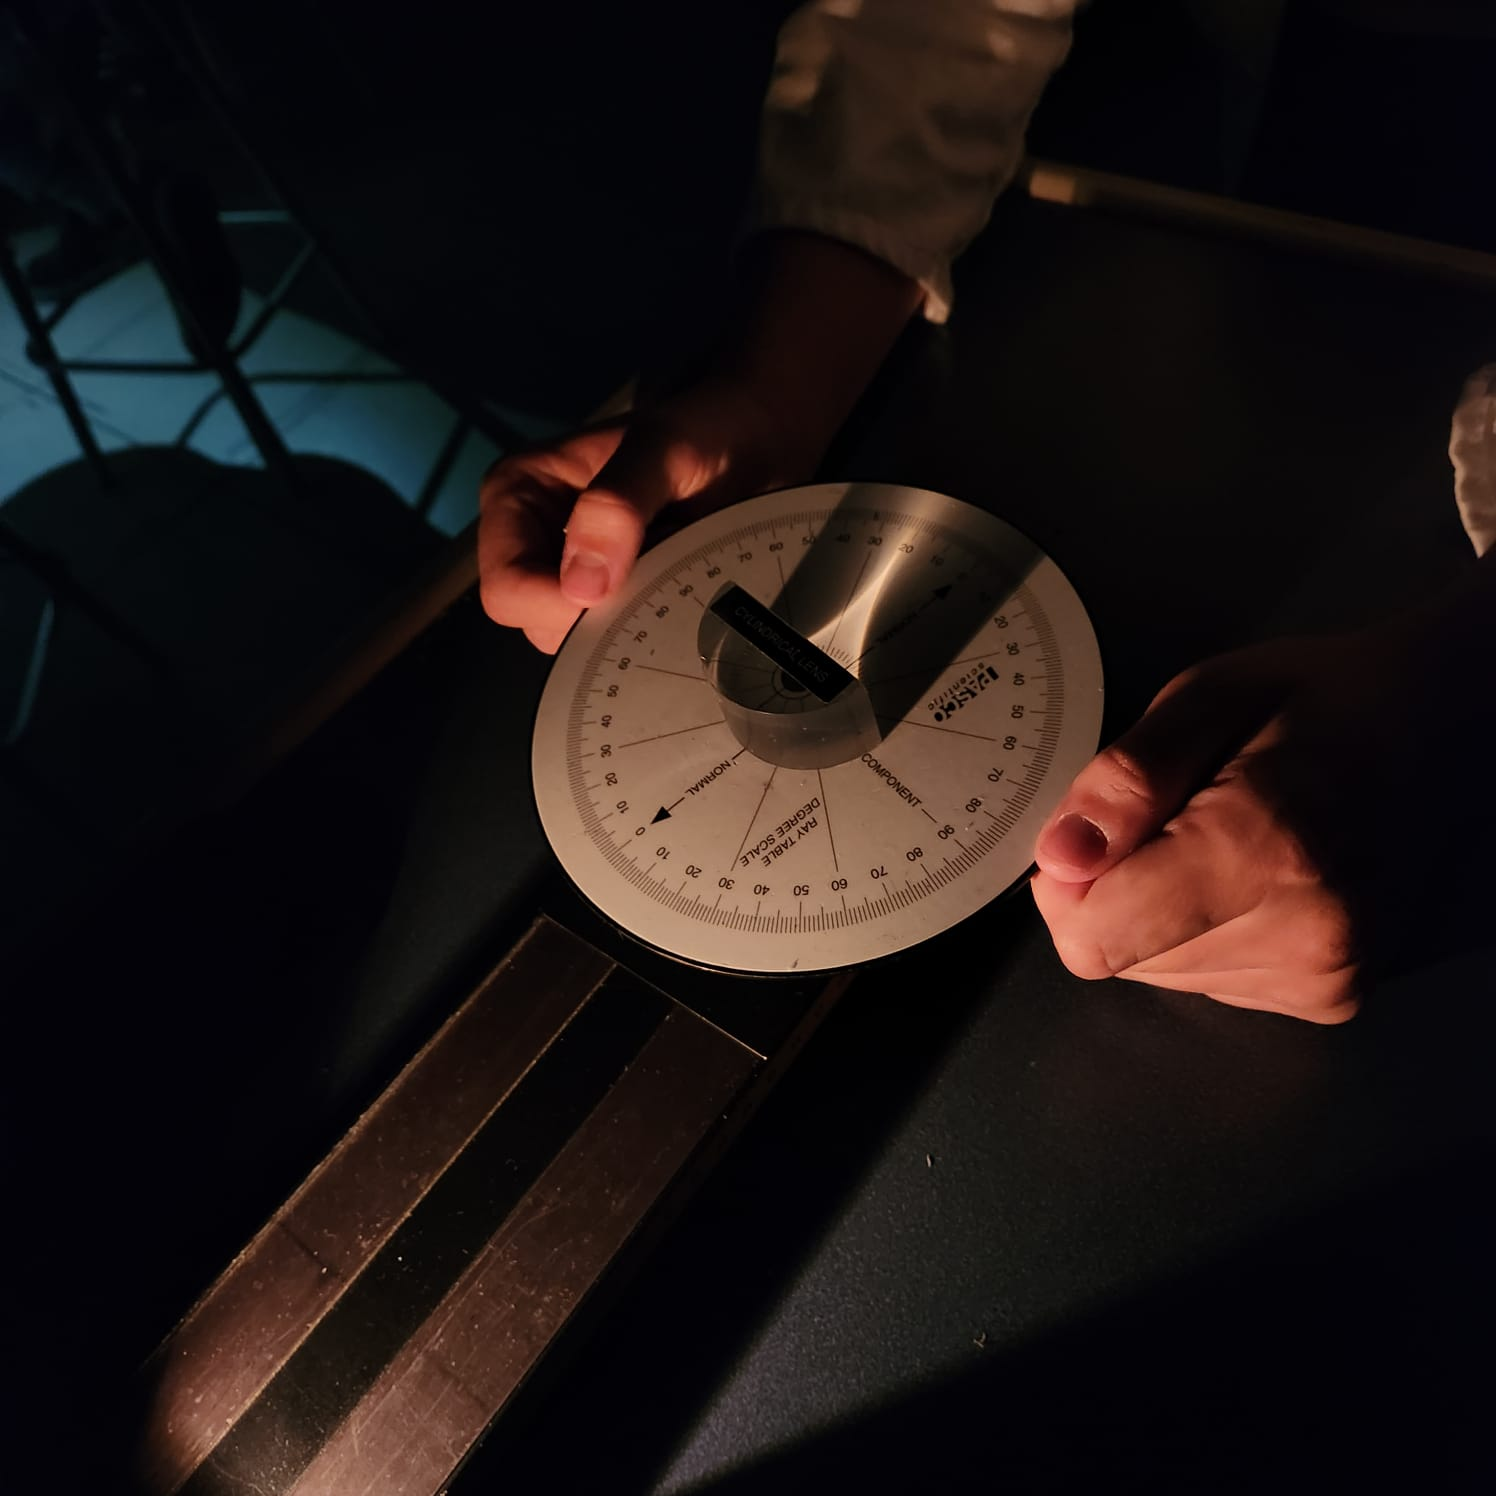
\includegraphics[width=\columnwidth]{mesa_rayos.jpg}
\captionof{figure}{Mesa de rayos con la lente cilíndrica colocada sobre el banco óptico.}
\label{fig:mesa}
\end{center}

La medición se hizo en dos partes. En la primera la luz entraba por la cara plana; giramos la mesa de 5 en 5 grados, desde 0 hasta 89, y para cada posición leímos el ángulo de incidencia y el ángulo del rayo que salía por la cara curva, ambos medidos desde la normal. En la figura \ref{fig:refraccion} se aprecia cómo el rayo se dobla al cruzar la lente.

\begin{center}
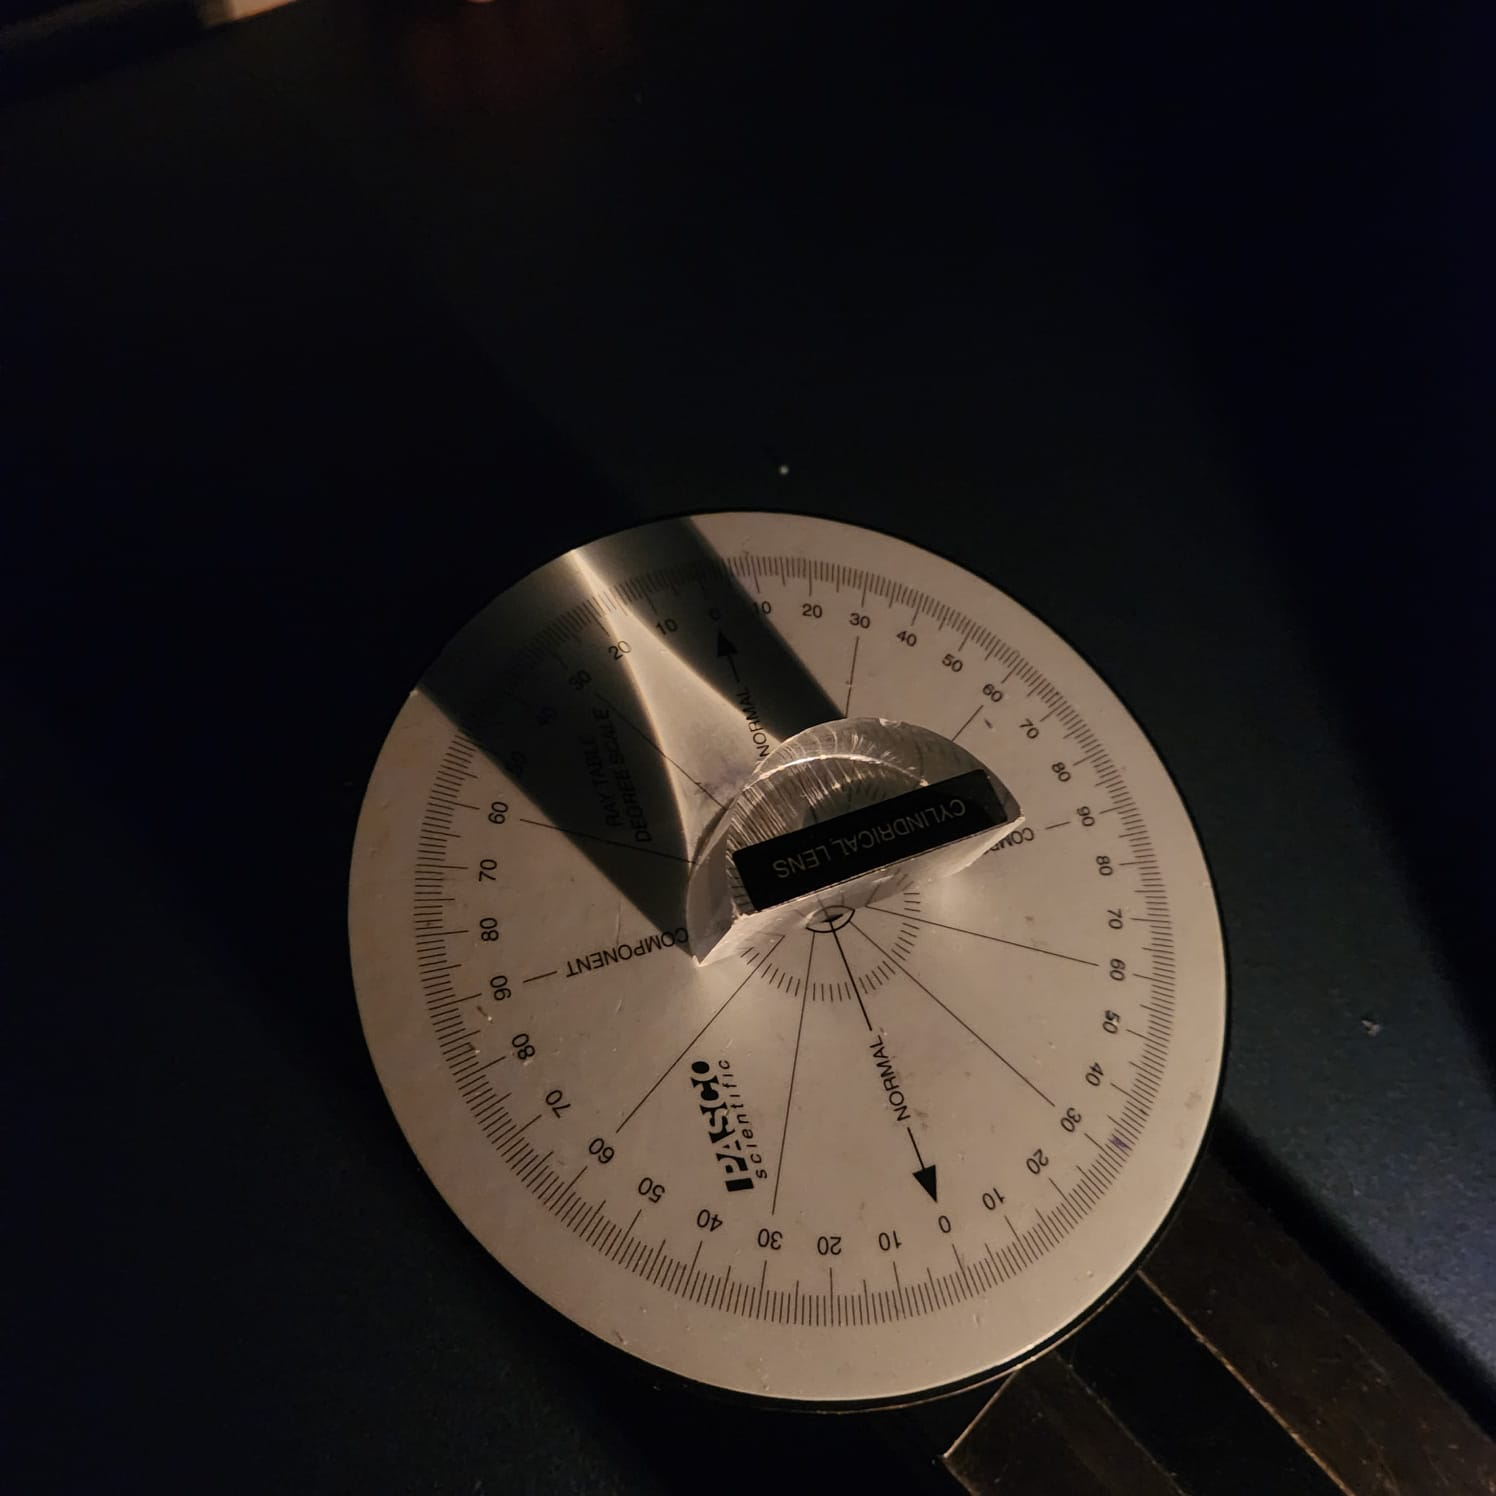
\includegraphics[width=\columnwidth]{refraccion_lente.jpg}
\captionof{figure}{Rayo de luz atravesando la lente de acrílico. Se nota el cambio de dirección respecto a la línea normal de la escala.}
\label{fig:refraccion}
\end{center}

En la segunda parte volteamos la lente para que la luz entrara por la cara curva y saliera por la plana, y repetimos el barrido de 0 a 90 grados. Esta vez pasó algo distinto: después de los 40 grados el rayo transmitido desapareció y lo único que quedó fue un rayo reflejado hacia dentro de la lente, cuyo ángulo también anotamos.
